\chapter{Protein Folding}

\say{\textit{la forma è l'immagine plastica	della funzione}}\footnote{\fullcite{ruffini1925fisiogenia}}\\

La correlazione tra forma e funzione si rivela fondamentale nel caso delle proteine. Un canale ionico neuronale permette il passaggio di ioni grazie alla sua forma a canale; una ferritina cattura e immagazzina gli ioni ferro grazie alla sua forma a sfera cava. 

\par Il ripiegamento delle proteine (\textit{protein folding}) è il processo di ripiegamento molecolare attraverso il quale a partire dalla sequenza lineare amminoacidica le proteine ottengono la loro struttura tridimensionale, chiamata forma \textit{nativa}, che permette loro di svolgere la relativa funzione biologica. 

\begin{figure}[htp]
	\centering
	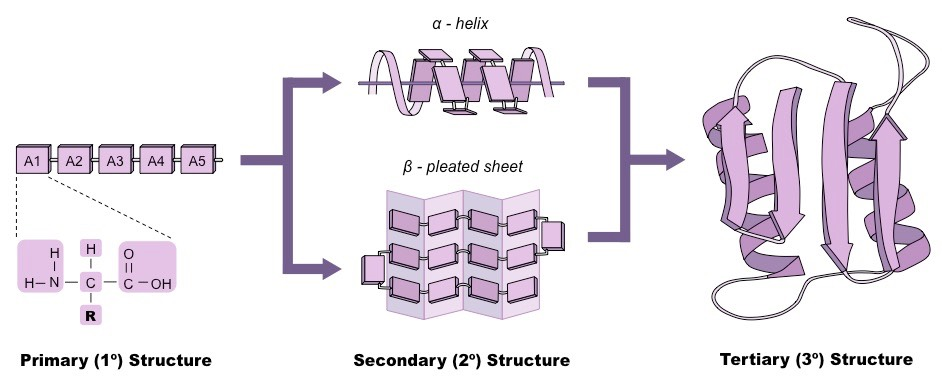
\includegraphics[scale=0.5]{images/protein-folding_med.jpeg}
	\caption{Protein folding: dagli amminoacidi alla struttura tridimensionale. Fonte: \cite{proteinStrucBioNinja}}
	\label{fig:protein-folding-bioninja}
\end{figure}


Il ripiegamento nella forma tridimensionale avviene spontaneamente sia durante la sintesi proteica nei ribosomi sia al termine di questa. Una specifica proteina si ripiegherà nello stesso modo e avrà la stessa struttura finale\footnote{ciò non è vero nel 100\% dei casi, alcune proteine possono avere più di una conformazione stabile per adempiere funzioni diverse (vedi la sezione \ref{sec:fold-switching-proteins}) e alcune proteine possono andare incontro a misfolding (vedi la sezione \ref{sec:assisted-folding})}.

\par La prima teoria del ripiegamento proteico è stata proposta negli anni venti del 20° secolo da Hsien Wu\supercite{wu1931studies}, in relazione al processo di denaturazione (vedi sezione \ref{sec:denaturazione}). È però Anfinsen, premio Nobel per la chimica, negli anni '60 a compiere un fondamentale passo nella comprensione del processo del ripiegamento proteico\supercite{anfinsen1972formation}. 


\section{Postulato di Anfinsen}
Il postulato di Anfinsen (conosciuto anche come \textit{dogma} o \textit{ipotesi termodinamica} di Anfinsen) afferma che la struttura nativa delle proteine (almeno quelle globulari) è determinata solamente dalla sequenza di amminoacidi di cui sono costituite. In altri termini: la struttura nativa, in ambiente fisiologico standard, corrisponde a quella struttura unica, stabile e cineticamente accessibile avente \textit{minima energia libera}. 

\begin{figure}[h]
	\centering
	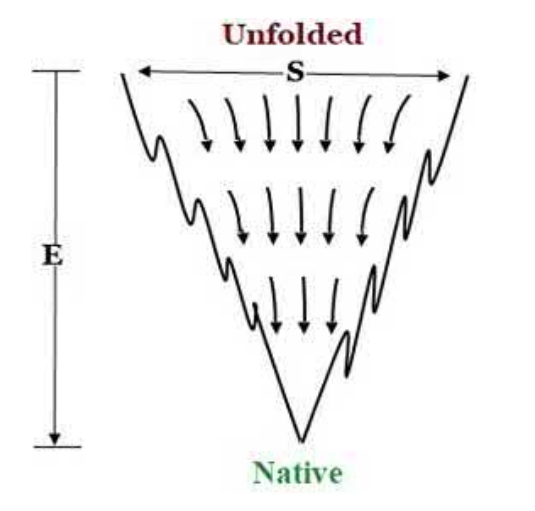
\includegraphics[scale=0.3]{images/funnel-folding.png}
	\caption{Un "panorama" idealizzato dell'energia libera a forma di imbuto. E=energia, S=entropia. Fonte: \cite{pal2019fundamentals}}
	\label{fig:funnel}
\end{figure}

Vi sono quindi 3 condizioni:

\begin{enumerate}
	\item \textit{unicità}, la sequenza non deve possedere altre configurazioni dotate di energia libera comparabile
	\item \textit{stabilità}, piccoli cambiamenti nell'ambiente circostante non possono produrre cambiamenti nella configurazione a energia minima. Ciò può essere descritto come una superficie parabolica di energia libera con lo stato nativo corrispondente al punto di minimo (visivamente simile ad un imbuto, vedi fig.\ref{fig:funnel}); la superficie di energia libera nelle vicinanze dello stato nativo deve essere abbastanza ripida ed elevata
	\item \textit{accessibilità cinetica}, il percorso nella superficie di energia libera dallo stato \textit{unfolded} a \textit{folded} deve essere ragionevolemente piano
\end{enumerate}


\subsection{Esperimento di Anfinsen}
L'esperimento, compiuto nel 1957\supercite{anfinsen1961kinetics}, consisteva nella denaturazione e rinaturazione della ribonucleasi A, dimostrando che il secondo processo era possibile senza agenti ausiliari. L'enzima in questione è formato da 124 amminoacidi, tra cui 8 cisteine che formano 4 ponti disolfuro ($-CH_{2}-\textbf{S-S}-CH_{2}-$). È stato usato un agente riducente per scindere questi ponti e l'urea per denaturare la proteina: questa non mostrava più alcuna attività enzimatica. A questo punto se l'urea era rimossa prima, seguita dall'aggiunta di un agente ossidante per consentire ai ponti disolfuro di riformarsi, la ribonucleasi A riacquistava spontaneamente la sua struttura terziaria e il prodotto ottenuto risultava praticamente indistinguibile dalla proteina nativa di partenza, riottenendo piena attività biologica. 

\begin{figure}[h]
	\centering
	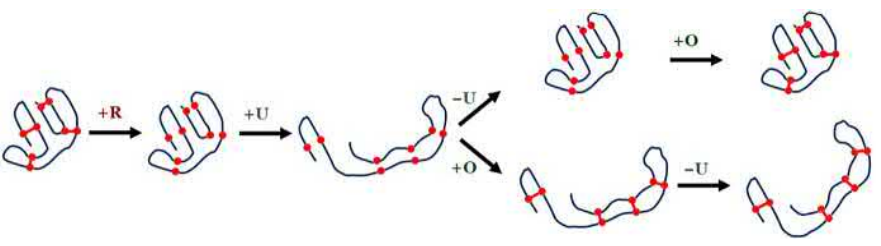
\includegraphics[scale=0.6]{images/anfinsen-experiment.png}
	\caption{Rappresentazione schematica dell'esperimento di Anfinsen. R=reducing agent, U=Urea, O=oxidizing agent, punti rossi=cisteina, linee rosse=ponti disolfuro. Fonte: \cite{pal2019fundamentals}}
	\label{fig:anfinsen-exp}
\end{figure}

I ponti disolfuro si riformano nella stessa posizione della proteina nativa nonostante ci siano 105 modi possibili per ricombinarli. Se invece veniva prima aggiunto l'agente ossidante e poi tolta l'urea il prodotto ottenuto era un miscuglio di molte delle possibili 105 configurazioni, raggiungendo solamente l'1\% dell'attività enzimatica.

\begin{figure}[!htb]
	\minipage{0.45\textwidth}
	\centering
	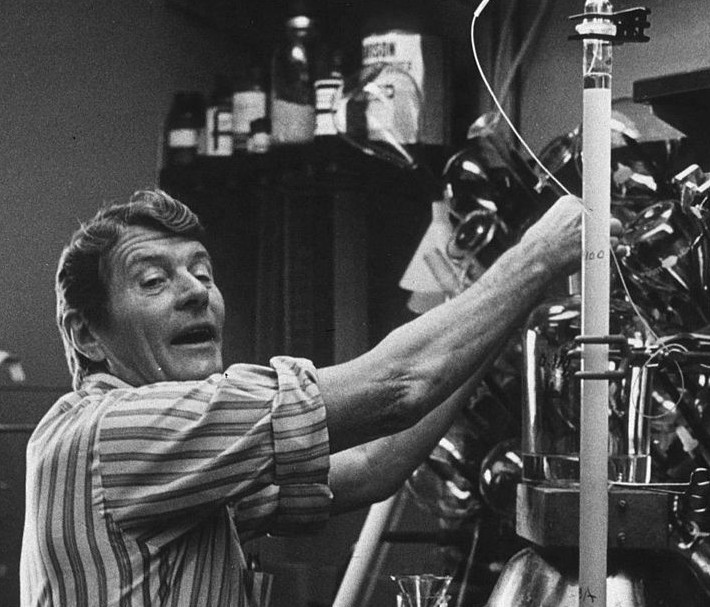
\includegraphics[scale=0.25]{images/anfinsen.jpg}
	\caption{C.B. Anfinsen nel suo laboratorio. Fonte: \cite{anfinsenNIH}}
	\label{fig:anfinsen}
	\endminipage\hfill
	\minipage{0.5\textwidth}
	\centering
	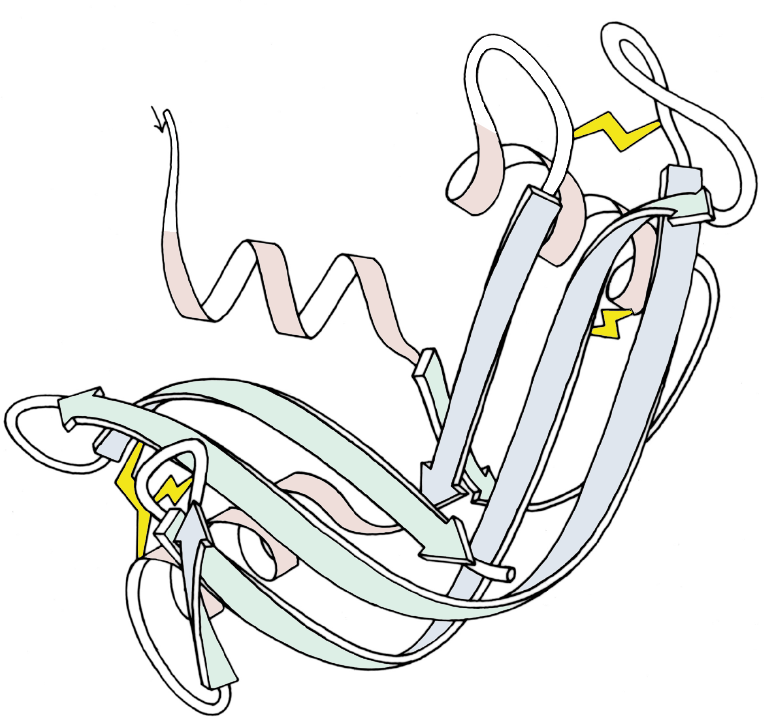
\includegraphics[scale=0.2]{images/RibonucleaseA_SS_paleRib.png}
	\caption{Ribonucleasi A, rappresentazione a nastro. In giallo i ponti disolfuro, rosa le $\alpha$-eliche, verde e azzurro i $\beta$-foglietti. Fonte \cite{ribonucleasi-file}}
	\label{fig:ribonucleasi}
	\endminipage\hfill
\end{figure}

\subsection{Denaturazione} \label{sec:denaturazione}
La denaturazione delle proteine è il fenomeno relativo all'alterazione della struttura nativa dovuto a variazioni di temperatura, pH o contatto con determinate sostanze chimiche. La denaturazione è un processo che porta alla perdita di ordine e quindi ad un aumento di entropia. La struttura primaria rimane invariata, data la stabilità dei legami peptidici. A causa della denaturazione le proteine perdono la loro funzione biologica e possono esporre e rendere reattivi alcuni gruppi funzionali che possono causare l'aggregazione di più proteine. Può avvenire che una volta rimosso l’agente denaturante la proteina ritorni allo stato di partenza (\textit{rinaturazione}) ma spesso il processo è irreversibile.

\begin{figure}[h]
	\centering
	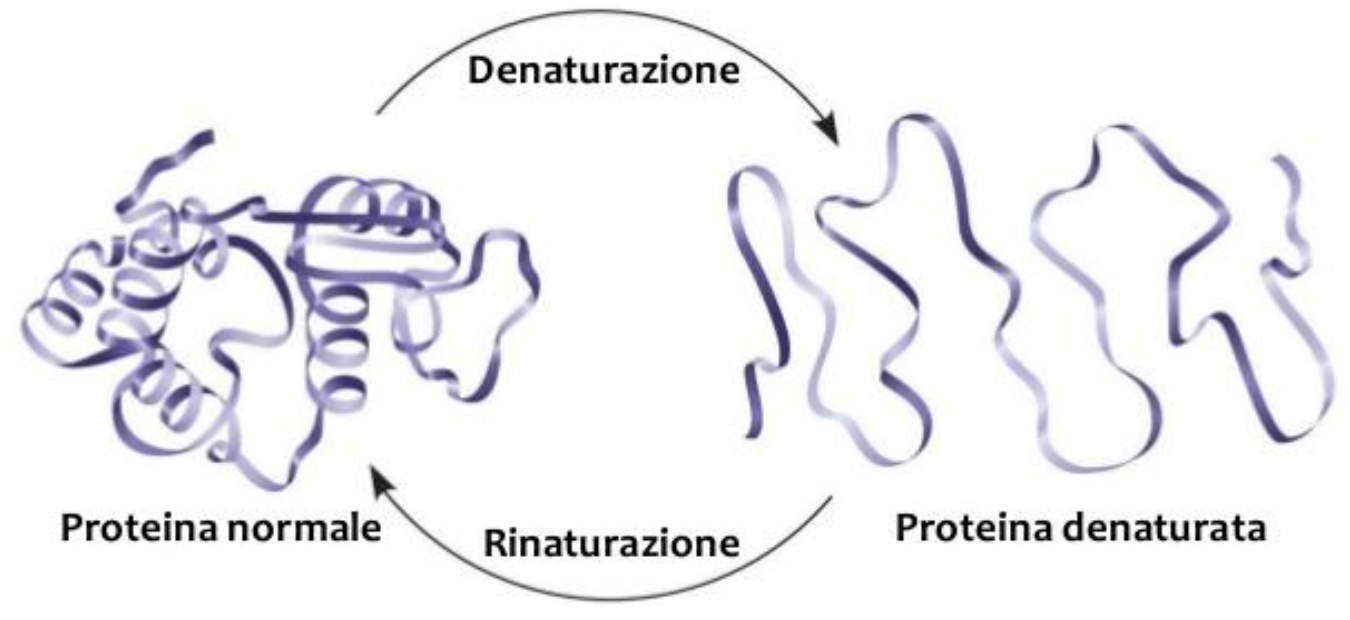
\includegraphics[scale=0.3]{images/denaturazione-rina.png}
	\caption{Denaturazione e rinaturazione. Fonte: \cite{campbell}}
	\label{fig:denaturazione}
\end{figure}

\par La proprietà di certe sostanze chimiche (es. urea) di denaturare una molecola proteica si deve alla loro capacità di legare transientemente, attraverso legami deboli, come ad esempio legami idrogeno, i residui amminoacidici costituenti la proteina. Questi legami vengono termodinamicamente preferiti a quelli intramolecolari o intermolecolari con l'acqua. Ciò comporta l'impossibilità per la proteina di mantenere la propria struttura tridimensionale e quindi questa si denatura. 

\par Applicazioni nella vita quotidiana di questo fenomeno sono la cottura dei cibi (basti pensare all'albumina nell'uovo) e la permanente ai capelli (denaturazione dell' $\alpha$-cheratina, rompendo e riformando ponti disolfuro). 


\section{Struttura delle proteine}
Da un punto di vista chimico le proteine sono di gran lunga, tra quelle conosciute, le molecole strutturalmente più complesse e sofisticate funzionalmente. È possibile studiare la loro struttura individuando successivi livelli di organizzazione:

\begin{figure}[!htp]
	\centering
	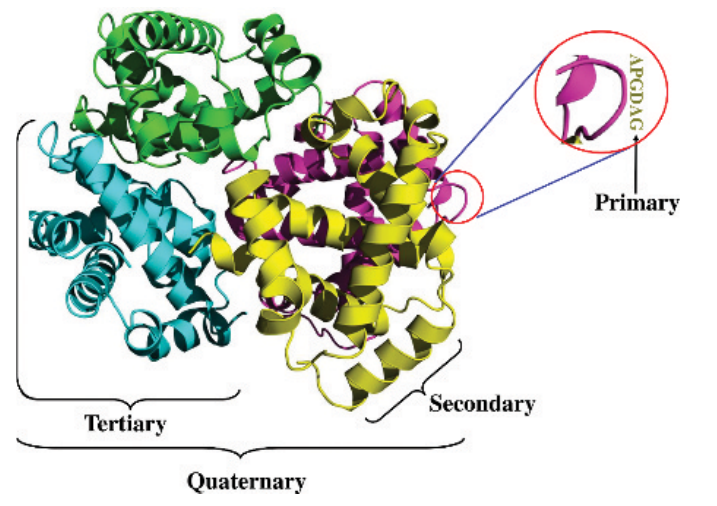
\includegraphics[scale=0.4]{images/strutture-proteina.png}
	\caption{Giri e Loop. Fonte: \cite{kessel_ben-tal_2018}}
	\label{fig:strutture-proteine}
\end{figure}

\begin{itemize}
	\item \textit{struttura primaria}: la sequenza ordinata degli amminoacidi
	\item \textit{struttura secondaria}: regioni ripetitive locali stabilizzate da legami idrogeno tra atomi della backbone ($\alpha$-eliche e $\beta$-foglietti)
	\item \textit{struttura supersecondaria}: combinazione di strutture secondarie e connessioni (motivi, domini, loop, giri ...)
	\item \textit{struttura terziaria}: forma tridimensionale di una singola catena polipeptidica, risultante dalle interazioni dei residui
	\item \textit{struttura quaternaria}: forma finale di proteine "assemblate" da 2 o più catene polipeptidiche già ripiegate
\end{itemize}

Prima di passare ad analizzare ogni livello della struttura delle proteine è utile un veloce sguardo alle interazioni molecolari.

\subsection{Interazioni molecolari}

\begin{itemize}
	\item \textit{legame covalente}: prevede la compartecipazione di 2 elettroni di valenza fra più atomi ed è il tipo di legame più forte (kcal/mol). Due o più atomi tenuti insieme da legami covalenti formano una molecola
		\begin{itemize}
			\item \textit{elettronegatività}:
		\end{itemize}
		
	\item \textit{legami non covalenti}
		\begin{itemize}
			\item \textit{legame ionico}: l'atomo più elettronegativo strappa completamente un elettrone al suo compagno, si formano due ioni (uno positivo, \textit{catione} e uno negativo, \textit{anione})
			\item \textit{legame idrogeno}: un atomo di idrogeno si trova fra due atomi elettronegativi vicini; ad es. nell'acqua gli atomi di idrogeno (parzialmente positivi) si trovano fra due atomi di ossigeno (parzialmente negativi). L'idrogeno, legato a uno dei due atomi di ossigeno, permette all'altro di avvicinarsi e di stabilizzarsi
			\item \textit{interazioni di van der Waals}: nelle molecole apolari gli elettroni si possono accumulare in modo asimmetrico, formando regioni momentaneamente polari che permettono così una temporanea stabilizzazione fra molecole a breve distanza
		\end{itemize}
	\item \textit{effetto idrofobico}: 
	\item 
\end{itemize}
\begin{itemize}
	\item \textit{ponte disolfuro}, lo zolfo di una cisteina si lega allo zolfo della seconda cisteina.
\end{itemize}

• una forza dominante o tante piccole forze?\\
• Cambio di paradigma da metà anni ‘80\\

\subsubsection{Struttura primaria}
La struttura primaria delle proteine è la sequenza ordinata degli amminoacidi che ne determina la conformazione nativa. La posizione nella sequenza di specifici amminoacidi è un fattore fondamentale per la determinazione di quali porzioni della proteina andranno a legarsi formando globalmente la struttura finale. La nota importante, basata sul dogma di Anfinsen, è che la sequenza amminoacidica di ogni proteina contiene l'informazione che specifica sia la struttura nativa che la via per raggiungere quello stato. Questo comunque non vuol dire che strutture simili si ripieghino in modo simile.
	
\subsubsection{Struttura secondaria}

La struttura secondaria riguarda le regioni ripetitive locali stabilizzate da legami idrogeno tra atomi della backbone: ($\alpha$-eliche e $\beta$-foglietti).

\begin{figure}[h]
	\centering
	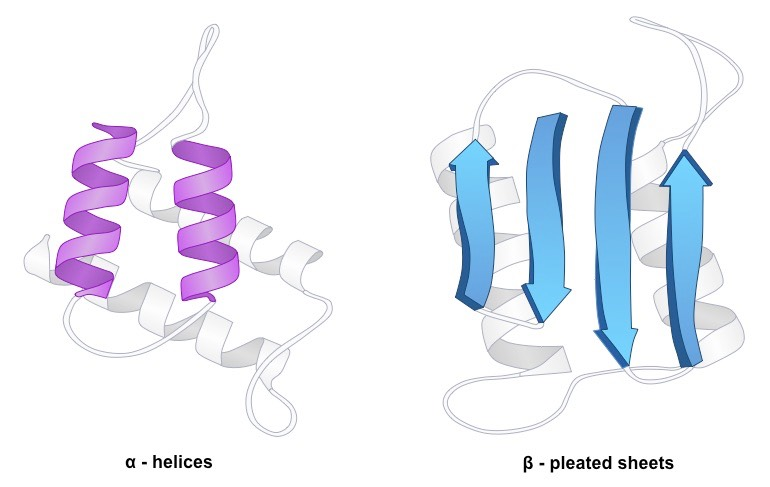
\includegraphics[scale=0.4]{images/secondary.jpeg}
	\caption{Struttura secondaria delle proteine, $\alpha$-eliche e $\beta$-foglietti. Fonte: \cite{proteinStrucBioNinja}}
	\label{fig:struttura-secondaria}
\end{figure}

Questo livello di organizzazione è una conseguenza dei legami a idrogeno tra gli amminoacidi appartenenti a una stessa catena, o tra gli amminoacidi di catene diverse.  All'interno della backbone del polipeptide gli atomi di ossigeno hanno una parziale carica negativa e gli atomi di idrogeno attaccati all'azoto hanno una parziale carica positiva perciò possono formarsi legami idrogeno fra questi atomi. Individualmente sarebbero deboli legami ma poiché sono ripetuti molte volte su di una regione relativamente lunga di una catena polipeptidica possono fare da supporto per una particolare conformazione.

\par Nella struttura ad $\alpha$-elica gli amminoacidi sono avvolti in una spirale tenuta insieme da legami idrogeno ogni 4 amminoacidi. Tra l’atomo di idrogeno legato all’azoto di ogni legame peptidico e l’ossigeno del gruppo carbossilico del legame peptidico sovrastante (che si trova appunto a distanza di quattro amminoacidi lungo la catena) si instaura un legame a idrogeno. Tuttavia se gli amminoacidi che si succedono lungo un tratto di catena proteica hanno gruppi R voluminosi, come avviene nella prolina, o gruppi R dotati della stessa carica elettrica, come avviene negli amminoacidi lisina e arginina, l’$\alpha$-elica non può formarsi, a causa delle forze di repulsione che si generano tra i residui. Alcune proteine fibrose, come l'$\alpha$-cheratina, la proteina strutturale dei capelli, la lana e le unghie hanno formazioni di $\alpha$-eliche sulla maggior parte della loro lunghezza.


\begin{figure}[!htp]
	\centering
	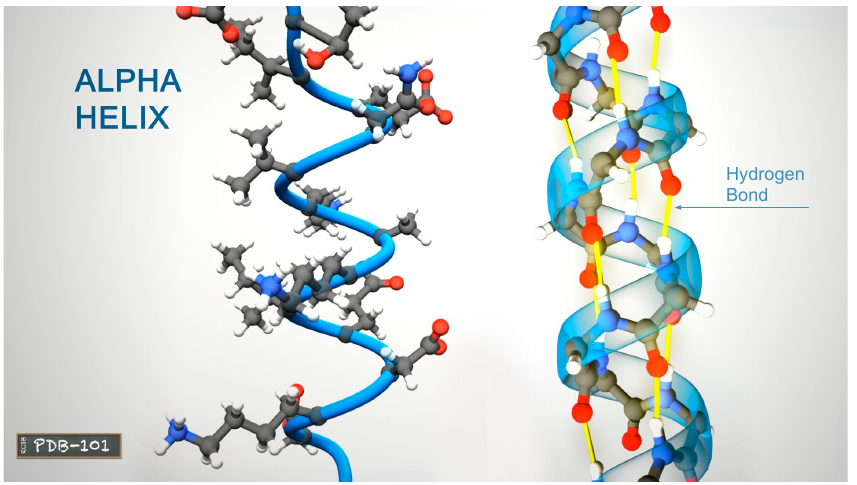
\includegraphics[scale=0.4]{images/alpha-helix.png}
	\caption{elica. Fonte: \cite{ProteinRCSB}}
	\label{fig:alpha-helix}
\end{figure}


\begin{figure}[!htp]
	\centering
	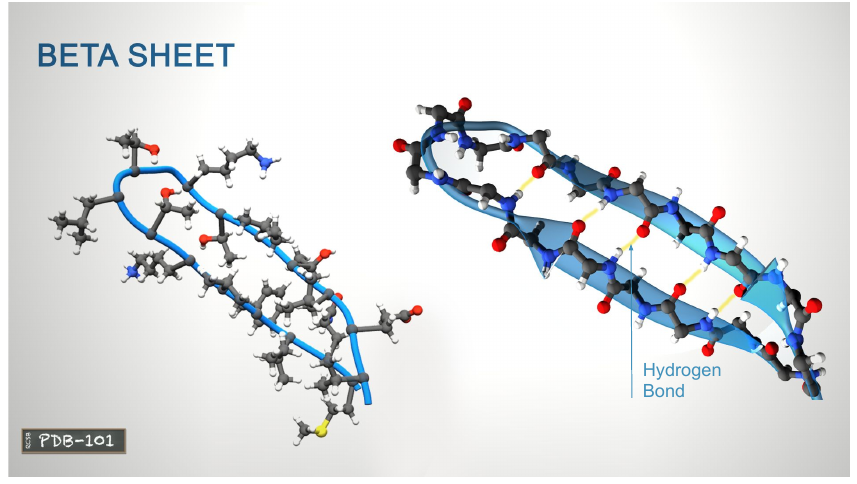
\includegraphics[scale=0.4]{images/beta-sheet.png}
	\caption{foglietto. Fonte: \cite{ProteinRCSB}}
	\label{fig:beta-sheet}
\end{figure}

\begin{figure}[!htb]
	\minipage{0.5\textwidth}
	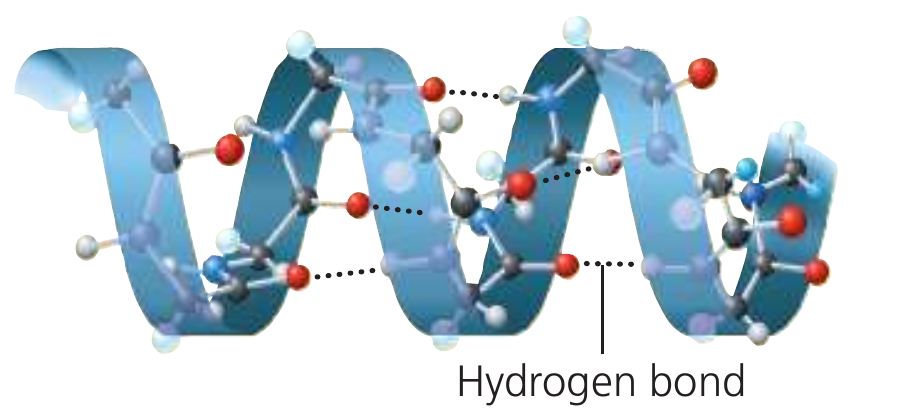
\includegraphics[scale=0.34]{images/eliche.png}
	\caption{Regione di $\alpha$-elica. Fonte: \cite{campbell}}
	\label{fig:eliche}
	\endminipage\hfill
	\minipage{0.5\textwidth}
	\centering
	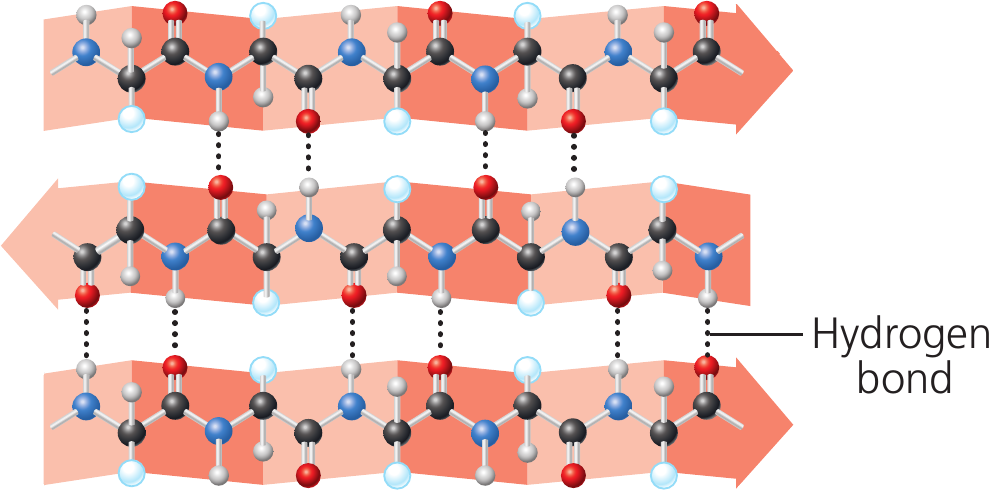
\includegraphics[scale=0.31]{images/foglietti.png}
	\caption{Una regione di $\beta$-foglietto composto da $\beta$-filamenti adiacenti, spesso mostrati come una freccia pieghettata o piatta puntata in direzione C-terminus. Fonte \cite{campbell}}
	\label{fig:foglietti}
	\endminipage\hfill
\end{figure}

Altre proteine fibrose sono invece dominate dai $\beta$-foglietti, come le proteine della seta ($\beta$-cheratina) e la tela prodotta dai ragni. In queste conformazioni due o più segmenti della catena polipeptidica giacenti lato su lato (chiamati $\beta$-filamenti) sono connessi da tre o più legami idrogeno. Si definisce $\beta$-filamento una sequenza peptidica di amminoacidi (tipicamente 5-10) che si dispone linearmente ed è in grado di formare legami idrogeno. Ciascuna delle catene è totalmente estesa e presenta una conformazione a zig-zag, dovuta alla geometria dei legami attorno a ciascun atomo di carbonio e di azoto nella catena. In questo caso, i legami a idrogeno si formano tra gli amminoacidi di due catene adiacenti. I gruppi amminici di uno scheletro peptidico formano legame con quelli carbossilici del filamento opposto. In ogni singolo filamento i residui si dispongono perpendicolarmente al piano del foglietto, puntando alternativamente verso l'alto e verso il basso.

\par Nella vita quotidiana, se tiriamo per i due estremi una fibra di lana questa si allunga: si stanno rompendo i legami idrogeno e le eliche si allontanano sempre di più, ma lasciando la presa i legami idrogeno si riformano e le eliche ricompaiono nella struttura. Se invece tiriamo la seta si può osservare che non è elastica: i foglietti di cui è composta la sua struttura non sono smantellabili senza rompere anche i legami covalenti della backbone.


\subsubsection{Struttura supersecondaria: Motivi, Domini, Loop, Giri ...}
La struttura supersecondaria è riferita alle combinazioni spaziali di strutture secondarie in conformazioni più complesse e alle connessioni che li uniscono. Può essere considerata come esempio di struttura supersecondaria la triplice elica allungata del collagene.

\par I \textit{motivi} (motifs) e \textit{domini} (domains) sono regioni tridimensionali della catena polipeptidica formate da differenti strutture secondarie adibite a svolgere una determinata funzione per la proteina di cui fanno parte. Tuttavia sono differenti in quanto i motivi non mantengono la loro forma se separati dalla proteina laddove i domini la mantengono. Questo perché i motivi e il resto della proteina sono più vicini e si vengono così a formare legami idrogeno che permettono ai motivi di mantenere la struttura. I domini sono sì legati alla backbone della proteina ma non abbastanza vicini alla restante parte della formazione proteica da stabilire legami, pertanto se vengono separati non perdono la loro struttura e possono mantenere la loro funzione.

\par Più in generale un \textit{motivo strutturale} è una struttura tridimensionale comune che appare in una varietà di molecole differenti ed evoluzionisticamente scollegate.

\begin{figure}[!htp]
	\centering
	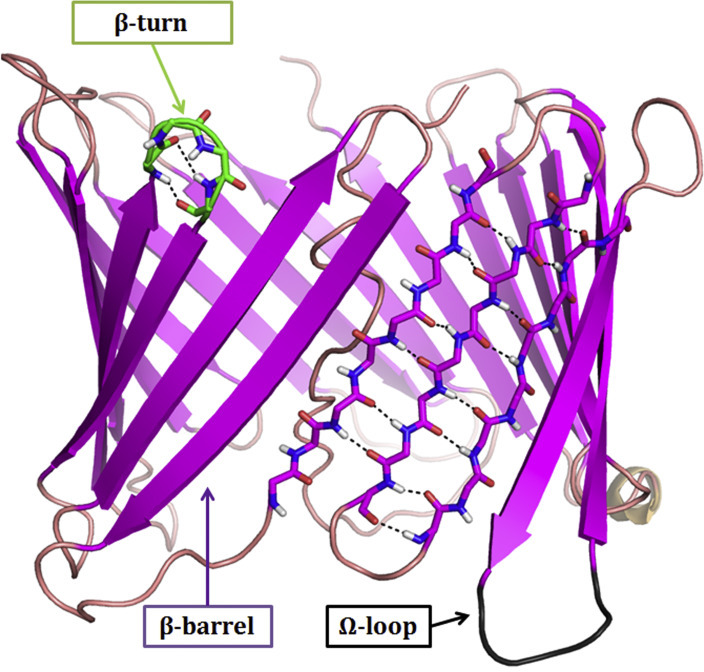
\includegraphics[scale=1.1]{images/turn-loop.jpg}
	\caption{Giri e Loop. Fonte: \cite{MURRAY2017477}}
	\label{fig:turn-loops}
\end{figure}


\par \textit{Giri} e \textit{loop} causano cambi di direzione alla backbone della proteina
Protein loops are patternless regions which connect two regular secondary structures. They are generally located on the protein's surface in solvent exposed areas and often play important roles, such as interacting with other biological objects. Despite the lack of patterns, loops are not completely random structures

\par Nelle strutture secondarie e terziarie si trovano spesso bruschi cambiamenti di direzione nella struttura: i \textit{giri} (turns). Queste nette svolte sono possibili grazie agli amminoacidi prolina e glicina. Il gruppo R della prolina si ripiega verso il gruppo amminico, distorcendo la catena naturalmente. Si forma però uno stretto spazio a causa del giro: l'amminoacido con gruppo R meno voluminoso è ovviamente la glicina ed è per questo che si trovano insieme nei giri.

\subsubsection{Struttura terziaria}
La struttura terziaria è la struttura tridimensionale globale risultante dalle interazioni tra i residui successivamente alle conformazioni locali della struttura secondaria ed è quindi la descrizione del risultato del processo di ripiegamento proteico. Un tipo di interazione importante è quella idrofobica che induce i residui non polari (e quindi idrofobici) a raggrupparsi al centro della catena polipeptidica, formando un nucleo idrofobico. La forma della proteina può venire rinforzata dai ponti disolfuro, legami covalenti fra due cisteine.

\begin{figure}[!htp]
	\centering
	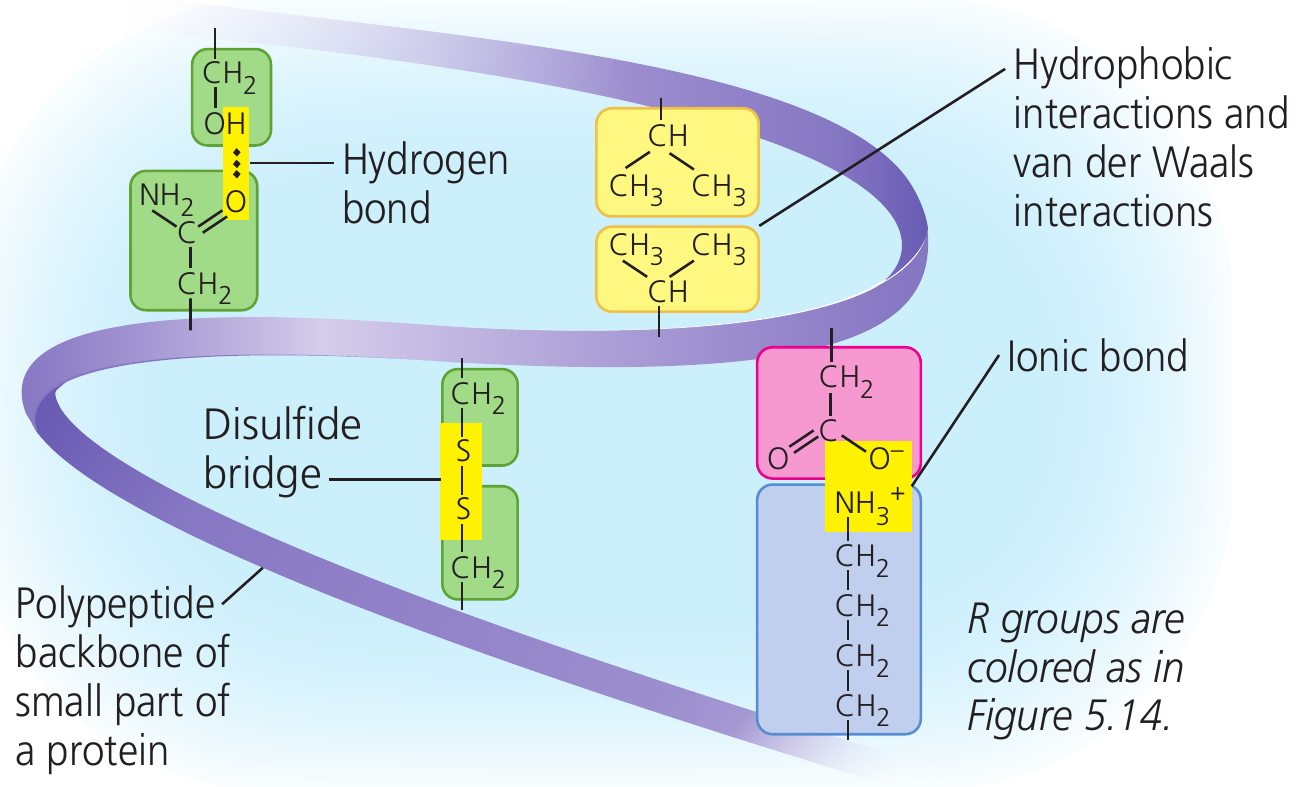
\includegraphics[scale=0.35]{images/interazioni-proteine.png}
	\caption{I diversi tipi di interazioni che possono contribuire alla struttura terziaria di una proteina. Fonte: \cite{campbell}}
	\label{fig:interazioni-proteine}
\end{figure}

\subsubsection{Struttura quaternaria}
La struttura quaternaria è la forma finale di proteine "assemblate" da 2 o più catene polipeptidiche già ripiegate. Il collagene ne è un esempio poiché è formata da 3 polipeptidi quasi interamente a spirale che si attorcigliano l'uno sull'altro formando un'elica tripla ancora più larga, dando alle lunghe fibre una grande forza. Un altro esempio è l'emoglobina, proteina globulare formata da 4 subunità polipeptidiche. Le strutture terziarie delle subunità non vengono alterate.

\begin{figure}[!htb]
	\centering
	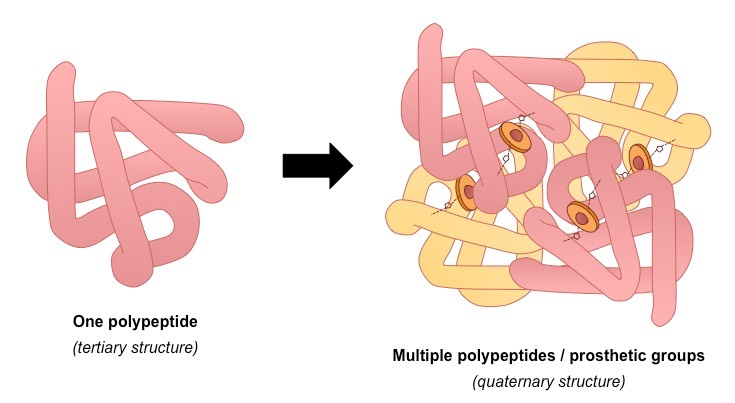
\includegraphics[scale=0.35]{images/quaternary-structure_med.jpeg}
	\caption{Rappresentazione di una struttura quaternaria composta da più polipeptidi e alcuni gruppi prostetica. Fonte \cite{proteinStrucBioNinja}}
	\label{fig:struttura-quaternaria}
\end{figure}

\subsection{Geometria dei legami?}

• Domini, Residui, Motivi, Giri, Loops, Turns\\

\section{Ripiegamento assistito} \label{sec:assisted-folding}
All'interno delle cellule le proteine più piccole si ripiegano indipendentemente, mentre proteine più grandi sono assistite principalmente da complessi chiamati \textit{chaperoni molecolari}. È  importante notare che l'assistenza è cinetica in natura: non aggiunge nuove informazioni necessarie alla proteina per ripiegarsi, pertanto il dogma di Anfinsen non viene contraddetto. Ciò che fanno questi complessi è creare un ambiente nel quale le proteine possano ripiegarsi senza "distrazioni" dovute a interazioni con altre entità (ad esempio evitando l'aggregazione con altre proteine) e senza rimanere bloccate in conformazioni intermedie durante il loro percorso di ripiegamento. In poche parole sono misure di protezione della cellula. 

\begin{figure}[h]
	\centering
	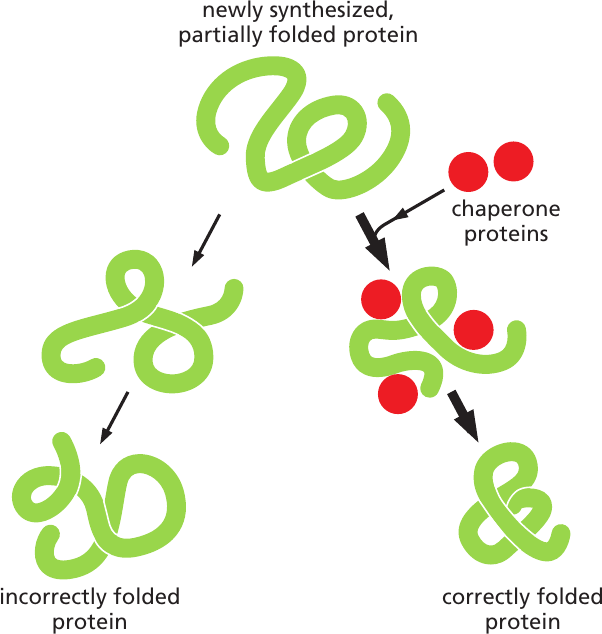
\includegraphics[scale=0.4]{images/chaperone-alberts.png}
	\caption{Schema della funzione dei chaperoni molecolari. Fonte: \cite{alberts2018essential}}
	\label{fig:chaperoni}
\end{figure}

Più in dettaglio i chaperoni molecolari svolgono le seguenti funzioni:
\begin{enumerate}
	\item assistono il corretto ripiegamento delle catene polipeptidiche (lunghe) appena sintetizzate
	\item dirigono l'assemblaggio di complessi multienzimatici
	\item donano una "seconda chance" a proteine danneggiate favorendone la rinaturazione
	\item partecipano nella parziale denaturazione durante il trasporto di proteine attraverso membrane di mitocondri o cloroplasti
\end{enumerate}

Tutti i compartimenti cellulari delle cellule eucariotiche (nucleo, citosol, reticolo endoplasmatico, mitocondri e cloroplasti) hanno il proprio set di chaperoni che assicura un corretto ripiegamento delle proteine. I chaperoni molecolari comprendono diverse famiglie di proteine altamente conservate, tra cui le Hsp (Heat shock protein), proteine espresse in grande quantità sotto condizioni di alto stress, per contrastarne l'effetto denaturante. Queste ultime sono state classificate in base al loro peso molecolare, ad es. Hsp60 dove "60" indica 60kDa. Le Hsp60 vengono chiamate anche \textit{chaperonine} e sono una famiglia di chaperoni molecolari a doppio anello che agiscono da "camera di isolamento" per il ripiegamento di altre proteine\supercite{ranson1998chaperonins}, famosa è la chaperonina procariotica GroEL (vedi fig.\ref{fig:groel}), che può essere assunta come modello di riferimento delle chaperonine. 

\begin{figure}[h]
	
\end{figure}

\begin{figure}[!htb]
	\minipage{0.35\textwidth}
	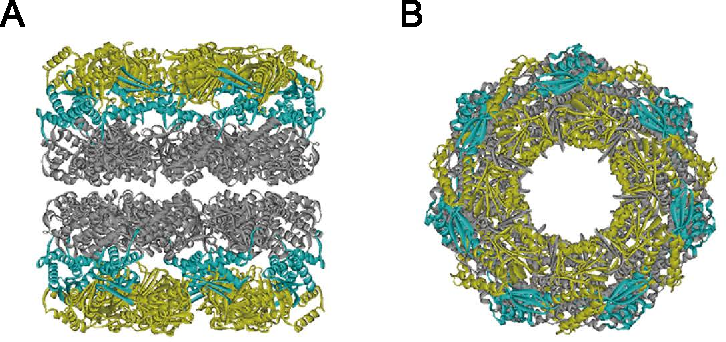
\includegraphics[scale=0.25]{images/groel.png}
	\caption{Strutture dei complessi GroEL e GroEL-GroES. (B) si può osservare la tipica forma ad anello. Fonte: \cite{Iizuka2016ChaperoninGU}}
	\label{fig:groel}
	\endminipage\hfill
	\minipage{0.6\textwidth}
	\centering
	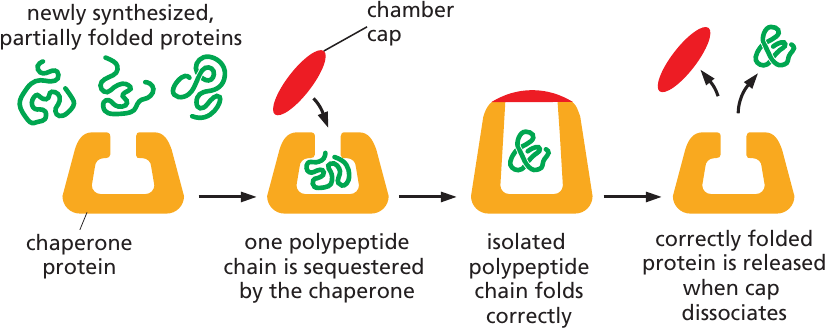
\includegraphics[scale=0.4]{images/chaperone-alberts-isolation.png}
	\caption{Rappresentazione schematica della funzione della camera di isolamento nelle chaperonine. Fonte \cite{alberts2018essential}}
	\label{fig:chaperone-camera}
	\endminipage\hfill
\end{figure}

Sebbene i mitocondri (e i cloroplasti) abbiano il loro genoma e creino le loro proteine, la maggior parte delle proteine che questi organelli usano sono codificate dai geni nel nucleo e importati dal citosol. Ogni proteina viene quindi parzialmente denaturata per effettuare il trasporto. I chaperoni molecolari all'interno di questi organelli aiutano a tirare le proteine attraverso le due membrane e a ripiegarle una volta all'interno\supercite{alberts2018essential}.


\subsection{Misfolding e malattie}

Il \textit{misfolding} è il fenomeno dell'errato ripiegamento di una proteina, ovvero quando una proteina non può raggiungere il suo stato nativo. Ciò può accadere per mutazioni alla sua sequenza amminoacidica, anche per un solo amminoacido differente (come nel caso dell'anemia falciforme) o per fattori esterni. Le proteine mal ripiegate tipicamente contengono $\beta$-foglietti organizzati in una struttura denominata cross-$\beta$, disposizione molto stabile e insolubile, generalmente resistente alla proteolisi. Il mal ripiegamento di alcune proteine può innescare ulteriori mal ripiegamenti e la conseguente accumulazione di proteine mal ripiegate in aggregati (od oligomeri) che possono guadagnare tossicità attraverso le interazioni intermolecolari. L'incremento dei livelli di proteine aggregate può portare alla formazione di \textit{amiloidi}, strutture fibrillari formate da deposizioni di materiale proteico insolubile. L'errato ripiegamento delle proteine è alla base quindi di molte patologie umane, definite malattie da misfolding, categorizzabili in due gruppi:

\begin{itemize}
	\item malattia causata dalla perdita o degradazione della proteina o dall'errato trasporto intracellulare
	\item malattie causate dall'accumulo, intra od extra-cellulare, di proteine aggregate (ad esempio le malattie da prione)
\end{itemize}

Molti tipi di tumore diventano chemio-resistenti perché iper-esprimono alcune Hsp, come la Hsp70 e la Hsp90. Le Hsp sono presenti anche in quantità elevatissime nel cervello dei pazienti con malattia di Alzheimer e morbo di Parkinson. Tuttavia si crede che la loro aumentata espressione non sia lesiva di per sé ma rappresenti piuttosto una risposta difensiva agli elevati livelli di stress che caratterizzano queste patologie. Ci sono molti morbi associati a mutazioni nei geni codificanti i chaperoni. Alterazioni genetiche delle chaperonine possono portare a patologie umane che in genere colpiscono molti organi ed apparati contemporaneamente \supercite{chaperoninaWiki}. \\

\par I \textit{prioni} (acronimo di "\textbf{pr}oteinaceous \textbf{i}nfective \textbf{on}ly particle") sono molecole di natura proteica con la capacità di trasmettere la propria forma mal ripiegata a varianti normali della stessa proteina. \footnote{I prioni sono stati studiati e denominati in questo modo dal premio Nobel per la medicina nel 1997 Stanley Prusiner\supercite{prusiner1998prion}} Il ruolo ipotizzato di una proteina come agente infettivo è in contrasto con tutti gli altri agenti infettivi conosciuti, come i viroidi, virus, batteri, funghi, parassiti: tutti contengono acidi nucleici (DNA, RNA o entrambi) mentre le proteine sono composte di soli amminoacidi.

\par I prioni formano amiloidi che si accumulano nei tessuti e sono associati a danni di questi e alla morte cellulare. I prioni sono attualmente considerati i più probabili agenti delle encefalopatie spongiformi trasmissibili (TSE) dei mammiferi. Nel \textit{morbo della mucca pazza} (encefalopatia spongiforme bovina), malattia neurologica degenerativa e irreversibile, vi è il ruolo di un prione a causare mal ripiegamenti di alcune proteine native causando la formazione di strutture amiloidi fatali (al microscopio le dense placche fibrose appaiono come buchi, da qui il caratteristico aspetto "a spugna"). Tutte le malattie da prione sono attualmente inguaribili e letali, con un periodo di incubazione che dura generalmente vari anni.

\par Gli aggregati di prioni sono stabili e questa stabilità strutturale consente loro di essere immuni alla maggior parte dei trattamenti conosciuti. L'organismo infettato non ha modo di degradarli: a differenza di virus e batteri i prioni rimangono intatti anche in presenza di trattamenti come sterilizzazione, forti dosi di radiazioni ionizzanti, uso di formaldeide, varechina, acqua bollente e a differenza delle altre proteine sono resistenti alla maggior parte delle proteasi.

\par La proteina di cui sono fatti i prioni, \textit{PrP} (protease-resistant-protein, Pr per \textbf{pr}ione, e P per \textbf{p}roteina), si trova in tutto il corpo, anche negli individui sani, ed è altamente conservata nei mammiferi. Tuttavia, la PrP trovata nel materiale infettante ha una struttura diversa. Nell'uomo la PrP$^{c}$(\textbf{c}ellulare, forma normale) è codificata da un solo gene, PRNP. La PrP$^{sc}$(\textbf{sc}rapie, forma patologica) differisce dalla proteina naturale PrP$^{c}$ per la conformazione tridimensionale: la PrP$^{c}$ ha una struttura più aperta contenente 3 segmenti ad $\alpha$-eliche e pochi $\beta$-foglietti; la PrP$^{sc}$ invece ha una struttura più compatta e stabile e presenta un aumento di $\beta$-foglietti.

\begin{figure}[h]
	\centering
	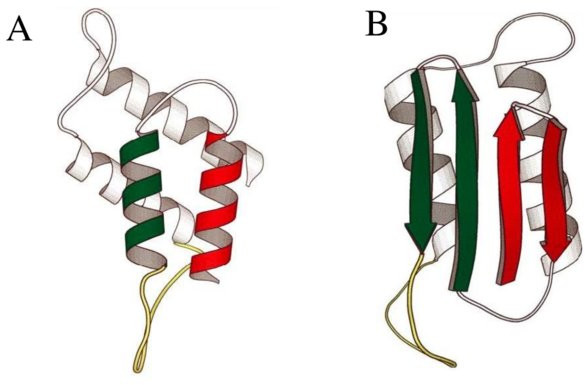
\includegraphics{images/PrPc.jpg}
	\caption{(A) Struttura della PrP$^{c}$. (B) Struttura della PrP$^{sc}$. Fonte: \cite{ruttkay2015prion}}
	\label{fig:PrPc}
\end{figure} 


\subsection{Controllo qualità e proteasomi}

L'uscita delle proteine dal reticolo endoplasmatico (RE) è controllata per assicurare la qualità delle proteine. Sebbene alcune proteine siano appositamente create e destinate a funzionare nel RE la maggior parte delle proteine che entrano nel RE sono destinate ad altri luoghi. Queste vengono impacchettate nelle vescicole di trasporto e gemmano per fondersi con l'apparato del Golgi. Ma l'uscita dal RE è altamente selettiva: le proteine che falliscono a ripiegarsi nella forma nativa e quelle che non si assemblano correttamente sono attivamente conservate nel RE attraverso i legami con i chaperoni molecolari che risiedono lì. Questi trattengono le proteine nel RE finché non si verifica il corretto ripiegamento o assemblaggio. Se questo non si verifica o fallisce ancora le proteine sono esportate nel citosol dove sono degradate da un \textit{proteasoma}. Le proteine da degradare sono contraddistinte dal loro legame con l'ubiquitina\footnote{Per "la scoperta della degradazione delle proteine mediata da ubiquitina" è stato assegnato il Premio Nobel per la chimica del 2004 ad Aaron Ciechanover, Avram Hershko ed Irwin Rose.}.

\par Ad esempio molecole di anticorpi sono composte da 4 catene polipeptidiche che si assemblano in completi anticorpi nel RE. Gli anticorpi parzialmente assemblati sono conservati nel RE finché tutte e 4 le catene non sono pronte. Le molecole di anticorpi che falliscono ad assemblarsi vengono degradate.

\par Nonostante l'indubbia utilità di questo meccanismo di controllo a volte questo può rivelarsi dannoso per l'organismo. Ad esempio la mutazione predominante che causa la \textit{fibrosi cistica}, comune malattia genetica che comporta seri danni polmonari, produce una proteina di trasporto della membrana plasmatica leggermente mal ripiegata. Tuttavia questa potrebbe funzionare normalmente se raggiungesse la membrana plasmatica ma viene bloccata nel RE e successivamente degradata\supercite{alberts2018essential} (per usare una metafora si può immaginare la situazione di un condannato alla pena di morte innocente). Le conseguenze sono terribili. La nota da sottolineare è che in questa malattia la mutazione non causa un'inattivazione di una proteina importante ma la proteina attiva è scartata dalle cellule prima che questa possa avere l'opportunità di funzionare. \\

\par I proteasomi sono complessi di \textit{proteasi} (enzima in grado di catalizzare la rottura del legame peptidico delle proteine) che degradano le proteine mal ripiegate attraverso reazioni di \textit{proteolisi}. Sono presenti nelle cellule di tutti gli eucarioti e procarioti. La struttura e la funzione di questi complessi è altamente conservata.

\par A causa del ruolo dei proteasomi nella regolazione del ciclo cellulare e dell'apoptosi\footnote{Il termine \textit{apoptosi} indica una forma di morte cellulare programmata (un'auto-distruzione). Al contrario della necrosi, che è una forma di morte cellulare risultante da un acuto stress o trauma cellulare, l'apoptosi è portata avanti in modo ordinato e regolato, richiede consumo di energia (ATP) e generalmente porta a un vantaggio durante il ciclo vitale dell'organismo (è infatti chiamata da alcuni morte altruista o morte pulita). Durante il suo sviluppo, ad esempio, l'embrione umano presenta gli abbozzi di mani e piedi “palmati”: affinché le dita si differenzino, è necessario che le cellule che costituiscono le membrane interdigitali muoiano}, sono oggi un bersaglio rilevante nelle terapie antitumorali. Farmaci inibitori nella terapia antiretrovirale interferiscono con il ciclo replicativo del virus HIV proprio bloccando l'attività dell'enzima della proteasi.


\subsection{Unfolded protein response}

La dimensione del RE è controllato dalla "richiesta" per il ripiegamento delle proteine. Il meccanismo di controllo nel RE, eseguito dai chaperoni molecolari, può essere sopraffatto. Quando succede le proteine mal ripiegate si accumulano nel RE. 
Se l'accumulo è abbastanza grande, questo innesca un complesso programma chiamato \textit{unfolded protein response} (UPR). Questo programma incita la cellula a produrre più RE, inclusi più chaperoni molecolari, e altre proteine riguardanti il controllo qualità. L'UPR permette alla cellula di regolare la dimensione del RE per gestire propriamente il volume delle proteine in entrata. In alcuni casi tuttavia anche un RE espanso non riesce a gestire la richiesta e l'UPR indirizza la cellula verso l'\textit{apoptosi}.

\par Una situazione del genere può avvenire negli adulti in cui insorge il diabete. I tessuti diventano gradualmente resistenti all'effetto dell'insulina. Per compensare questa resistenza le cellule che secernono insulina nel pancreas ne producono ancora di più. Si arriva infine alla situazione in cui il loro RE arriva ad una capacità massima e viene innescato l'UPR e di conseguenza la morte cellulare. Col tempo sempre più cellule secernenti insulina sono eliminate e la richiesta per quelle sopravvissute aumenta rendendole sempre più vulnerabili a questo meccanismo, esacerbando ulteriormente la malattia\supercite{alberts2018essential}.

\section{Eccezioni al postulato di Anfinsen}

-- IDP [ soft computing articolo]---
The structure of some proteins is difficult to determine
for a simple reason: A growing body of biochemical research
has revealed that a significant number of proteins, or regions
of proteins, do not have a distinct 3-D structure until they
interact with a target protein or other molecule. Their flexibil-
ity and indefinite structure are important for their function,
which may require binding with different targets at different
times. These proteins, which may account for 20–30% of
mammalian proteins, are called intrinsically disordered proteins
and are the focus of current research.


\subsection{Intrinsically disordered proteins}

\subsection{Fold switching proteins} \label{sec:fold-switching-proteins}
Some proteins have multiple native structures, and change their fold based on some external factors. For example, the KaiB protein complex switches fold throughout the day, acting as a clock for cyanobacteria. It has been estimated that around 0.5–4\% of PDB proteins switch folds.[7] The switching between alternative structures is driven by interactions of the protein with small ligands or other proteins, by chemical modifications (such as phosphorylation) or by changed environmental conditions, such as temperature, pH or membrane potential. Each alternative structure may either correspond to the global minimum of free energy of the protein at the given conditions or be kinetically trapped in a higher local minimum of free energy.[8]


--- porter, youtube ---
“I study proteins and proteins have been thought to have one structure that has one function or fold. I'm studying this group of proteins called fold switching proteins. So, they can actually change their structures and their functions in response to changes in the cell. So, you can kind of imagine fold switching proteins are like a transformer where in one case the protein is like a robot that does one thing and then in another case, in response to changes in our bodies, it becomes a car and can do something else. And an advantage to this is it can respond really quickly to changes in our bodies

\subsection{box: Filosofia della scienza}


\section{Il problema del Protein Folding}
• cos’è il problema del protein folding: non solo la struttura finale\\
• 3 sottoproblemi: folding code, protein structure prediction e folding process\\
• le domande di principio del protein folding\\
- paradosso di Levinthal

Come accennato nella sezione \ref{sec:assisted-folding}, la malattia di Alzheimer, la fibrosi cistica e altre malattie neurodegenerative sono associateal mal ripiegamento delle proteine. La conoscenza dei fattori di mal ripiegamento e la comprensione dei processo di ripiegamento proteico potrebero aiutare nello sviluppo di cure per queste malattie. La conoscenza della struttura delle proteine fornisce un grande vantaggio per lo sviluppo di nuovi farmaci e il design di nuove proteine.


\subsection{Limiti al ripiegamento}
• Limiti al ripiegamento: angoli di tersione e piano di Ramachandran\\

\subsection{Energetica del ripiegamento}
• processo spontaneo: energia di Gibbs, entalpia, entropia\\


--- Biochemists now know the amino acid sequence for about
160 million proteins, with about 4.5–5 million added each
month, and the three-dimensional shape for about 40,000.
Researchers have tried to correlate the primary structure of
many proteins with their three-dimensional structure to dis-
cover the rules of protein folding. Unfortunately, however,
the protein-folding process is not that simple. Most proteins
probably go through several intermediate structures on their
way to a stable shape, and looking at the mature structure
does not reveal the stages of folding required to achieve that
form

-- strumenti [ soft computing articolo]---
Even when scientists have a correctly folded protein in
hand, determining its exact three-dimensional structure is
not simple, for a single protein has thousands of atoms. The
method most commonly used to determine the 3-D structure
of a protein is X-ray crystallography


\clearpage